\documentclass[../main]{subfiles}
\usepackage{subcaption}
    \setcounter{secnumdepth}{2}
    \chapter{提案手法}
        \section{全天球カメラに基づく通路認識手法}
        本研究は,全天球カメラから取得した画像に基づき,通路認識を行う手法の検証を行う.ここでいう通路認識とは,画像中に通路があるかどうかを検出するだけでなく,
        画像中に通路がある場合,その通路がどのタイプに属するのかといった,通路の情報を取得することである.また,本研究で扱う通路のタイプは\fref{figure::new_aisle_type}に
        示すような8種類である.

        \begin{figure}[H]
            \centering
            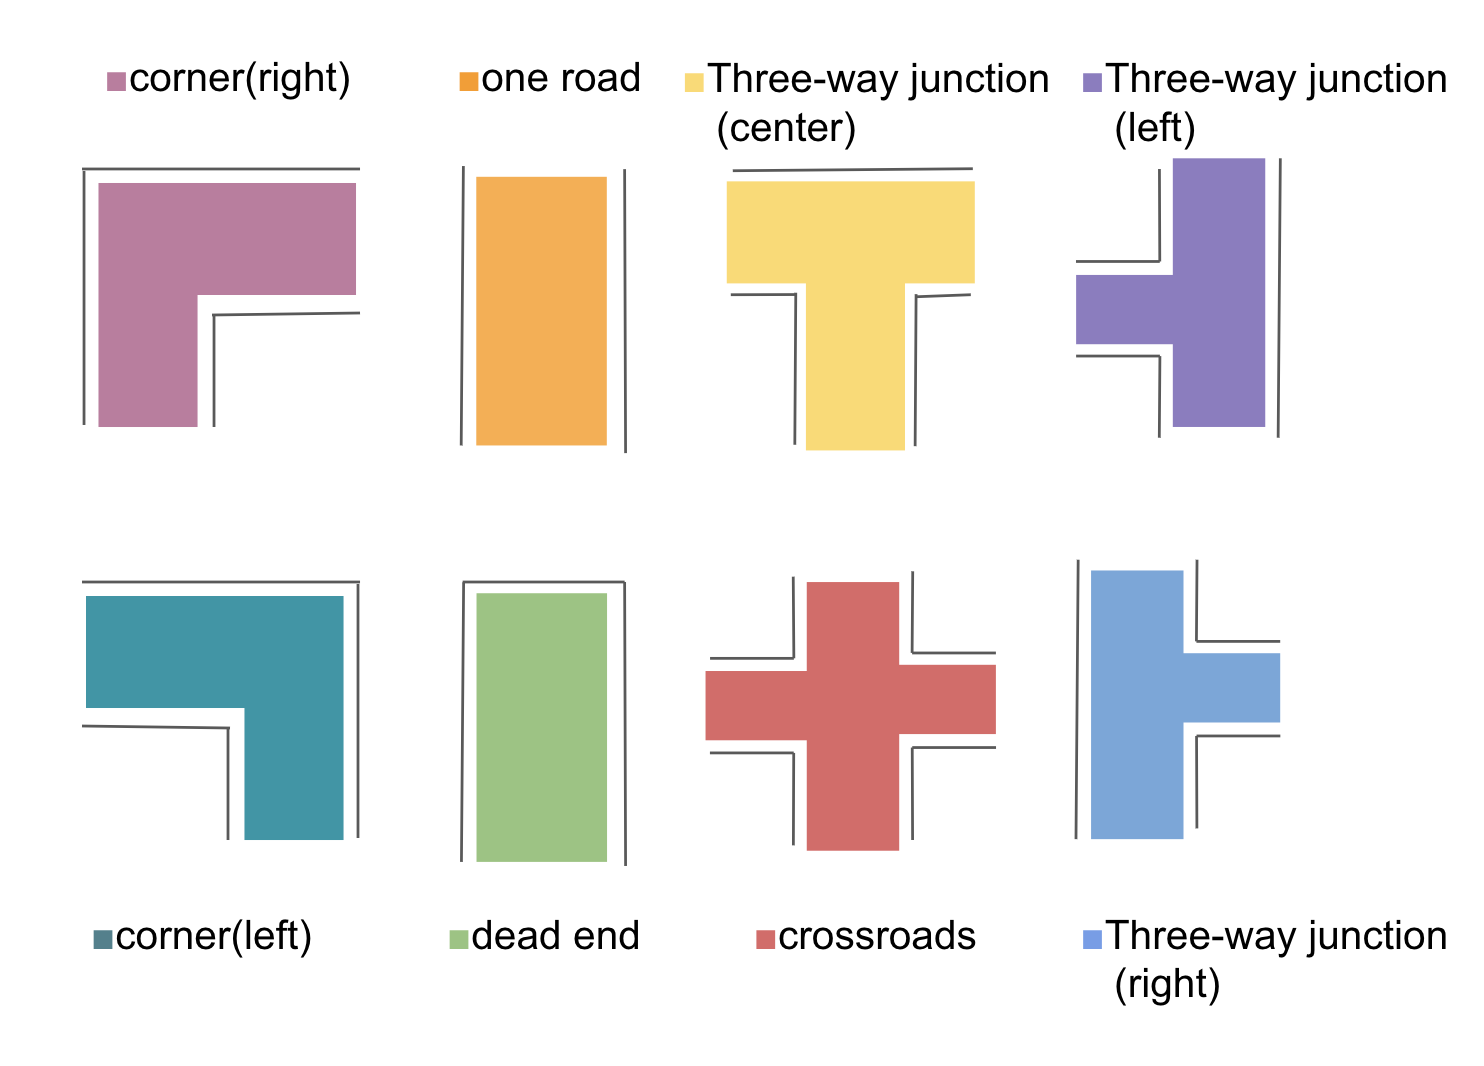
\includegraphics[width=10cm]{new_aisle_type.png}
            \label{figure::new_aisle_type}
            \caption{Type of passage.}
        \end{figure}
        
        \newpage

        本手法の通路認識の流れを\fref{figure::proposed_method_fig}に示す.
        まず,全天球カメラ画像のRGBデータをYOLOの入力とし,出力された情報をもとに画像中に通路があるかどうかを検出する.
        画像中に通路が検出された場合,バウンディングボックスにより得られる画像中の通路の座標に基づき,通路のタイプを決定する.

        \begin{figure}[H]
            \centering
            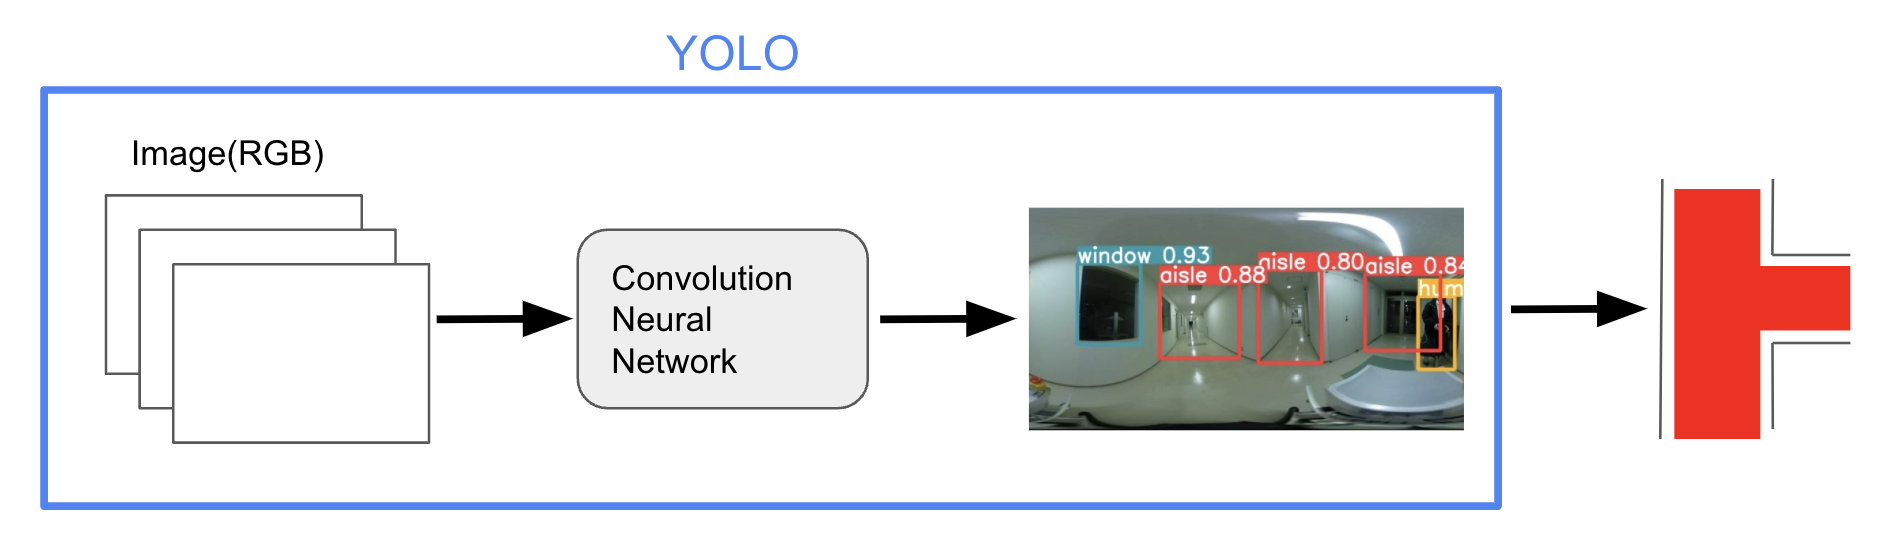
\includegraphics[width=15cm]{proposed_method2.png}
            \caption{Flow of passage recognition method.}
            \label{figure::proposed_method_fig}
            この例では,画像から通路が3つ検出されている.また,通路はロボットに対して\\
            前方,後方,右手側に検出されているため,タイプは三叉路であるということがわかる.
        \end{figure}

        \newpage
        
        全天球カメラにより得られた画像は,後方の通路が見切れ学習後の精度確認の段階で通路の認識がうまくできていなかったため,
        \fref{figure::image_proc_fig}に示すような画像の前処理を施した.
        YOLOの学習モデル作成のため,自作のデータセットを作成し,学習を行う.画像データは,実験環境として想定している
        本学の津田沼キャンパス2号館3階で実験につかうロボットに
        全天球カメラを取り付けて収集した.データセットの一例を\fref{figure::dataset_fig}に示す.
        また,データセットのクラスは\tref{table::datasets_table}の11クラスで設定した.
        先行研究では,8つの形状タイプの通路の認識を行なったため,本研究でも先行研究と同様の通路認識を行う.
        次に,YOLOの出力として得られた通路の情報に基づき,を参考にし,画像中の通路が認識された箇所を場合分けし,通路の形状を決定する.

        \begin{figure}[htbp]
            \begin{center}
                \begin{tabular}{c}
                \begin{minipage}{0.5\linewidth}
                 \begin{center}
                 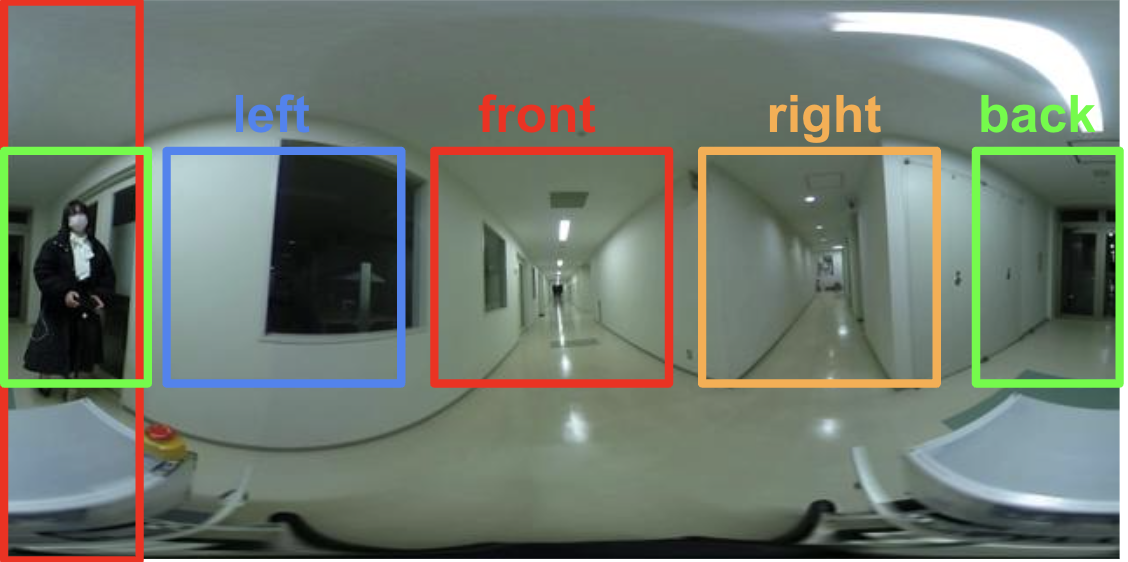
\includegraphics[clip, height=6cm]{no_processing.png}
                 \hspace{1.6cm}
                 \end{center}
                 \subcaption{Image before processing}
                \end{minipage}
                \begin{minipage}{0.5\linewidth}
                 \begin{center}
                 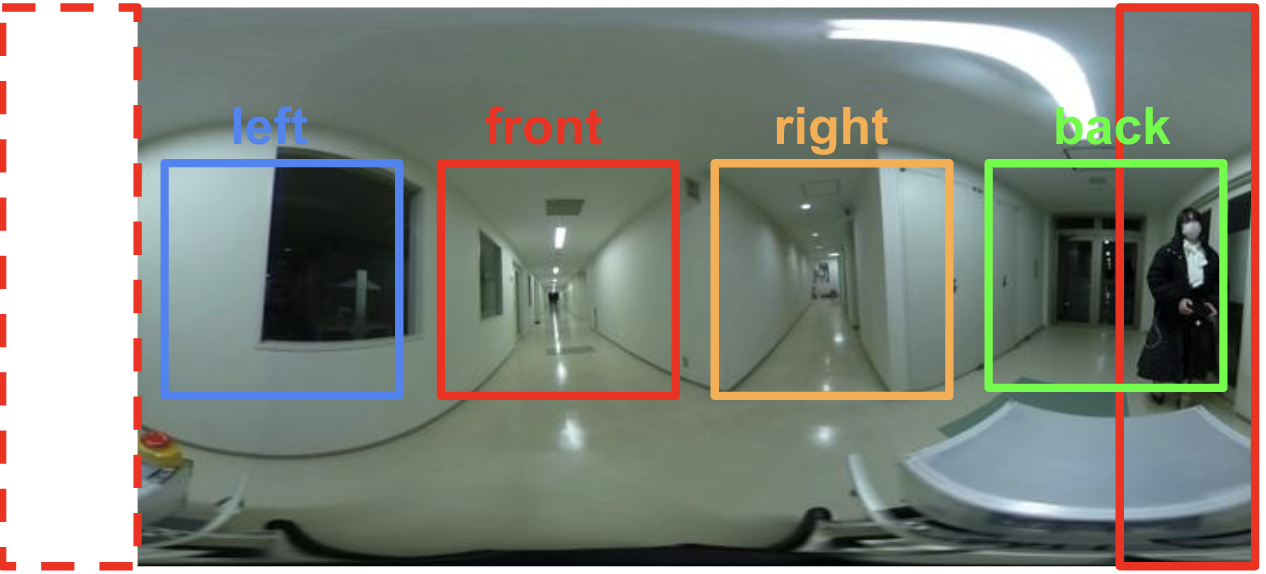
\includegraphics[clip, height=6cm]{after_processing.png}
                 \subcaption{Preprocessed image}
                 \end{center}
                \end{minipage}
                \end{tabular}
                \caption{Preprocessing of spherical camera images.}
            \end{center}
        \end{figure}

        \begin{figure}[H]
        \centering  
        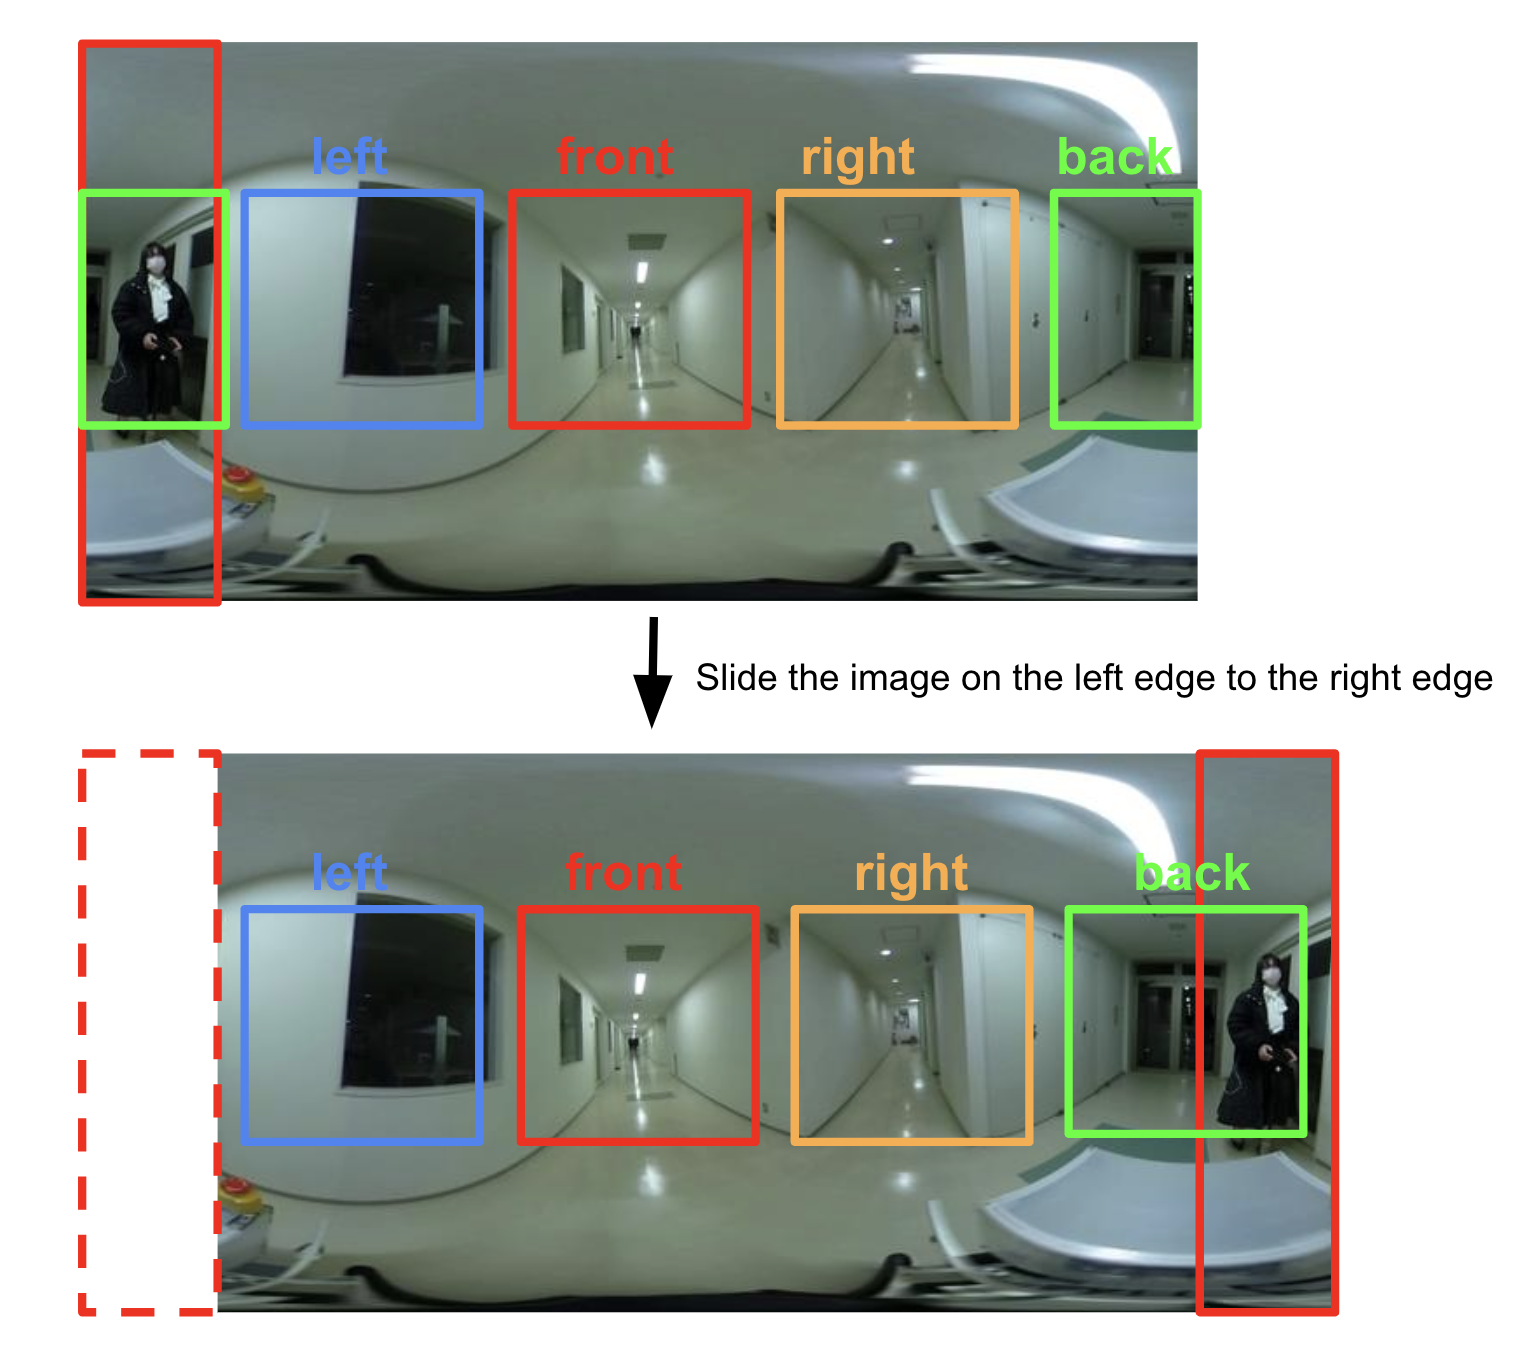
\includegraphics[width=15cm]{image_proc2.png}
        \caption{Preprocessing of spherical camera images.}
        \label{figure::image_proc_fig}
        \end{figure}

        \begin{figure}[H]
         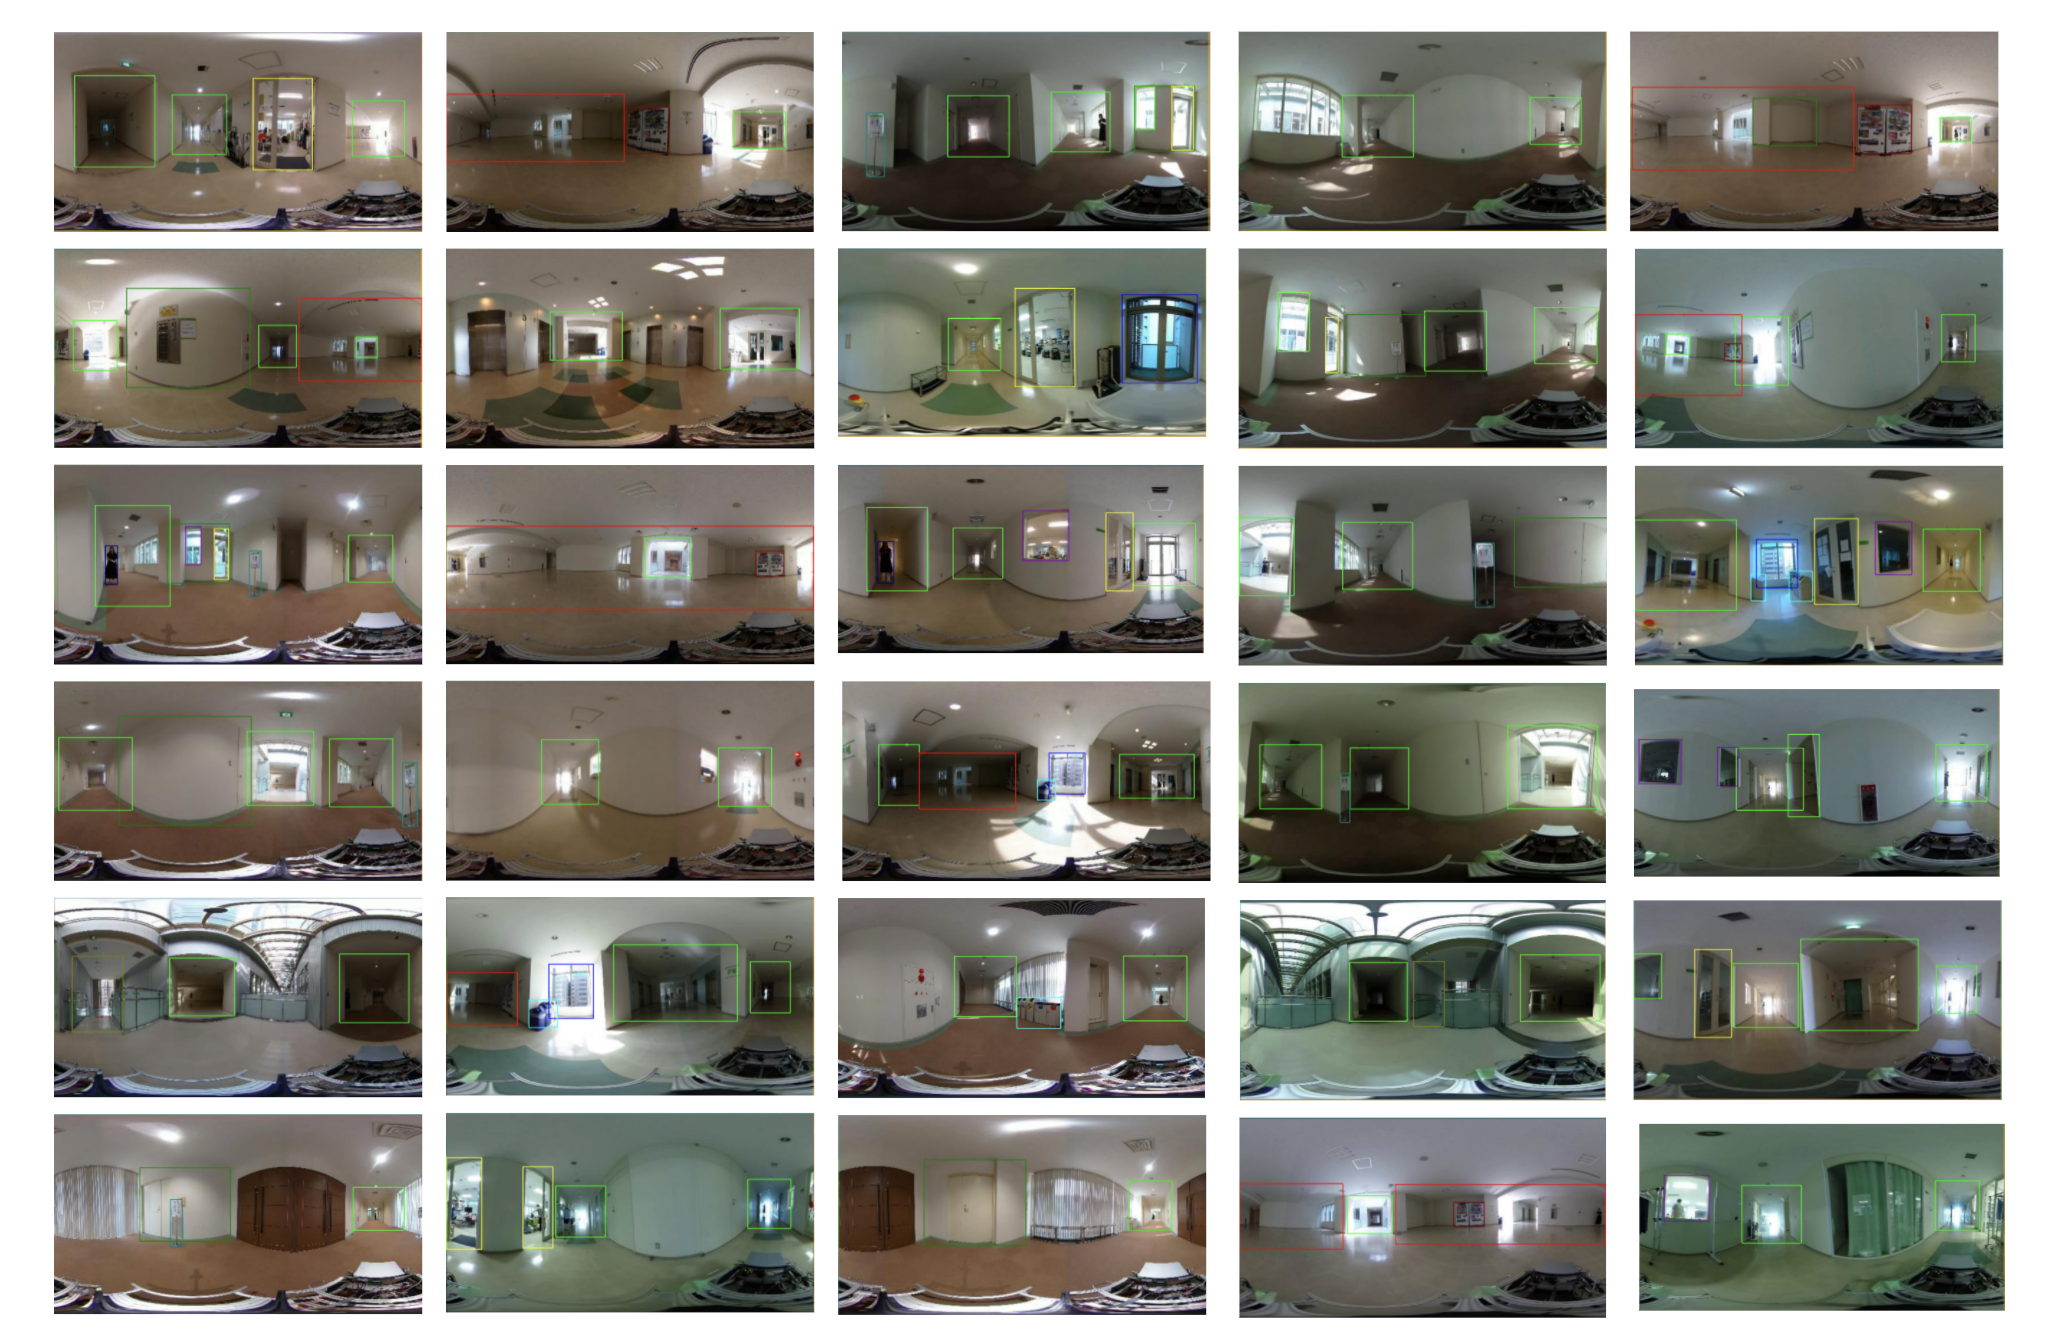
\includegraphics[width=15cm]{dataset_exp.png}
         \caption{An example of a dataset.}
         \label{figure::dataset_fig}
        \end{figure}

        \begin{table}[H]
            \caption{Class name to be labeled.}
            \centering
            \label{table::datasets_table}
            \begin{tabular}{lllll}
            \hline
            name of the class &  &  &  &  \\ 
            \hline \hline
            aisle             &  &  &  &  \\
            end               &  &  &  &  \\
            door\_end         &  &  &  &  \\
            human             &  &  &  &  \\
            door              &  &  &  &  \\
            step              &  &  &  &  \\
            square            &  &  &  &  \\
            vending\_machine  &  &  &  &  \\
            trash\_can        &  &  &  &  \\
            signboard         &  &  &  &  \\
            window            &  &  &  &  \\ 
            \hline
            \end{tabular}
        \end{table}
\end{document}